% document formatting
\documentclass[10pt]{article}
\usepackage[utf8]{inputenc}
\usepackage[left=1in,right=1in,top=1in,bottom=1in]{geometry}
\usepackage[T1]{fontenc}
\usepackage{xcolor}

% math symbols, etc.
\usepackage{amsmath, amsfonts, amssymb, amsthm}
\usepackage{dsfont}

% lists
\usepackage{enumerate, enumitem}
\usepackage{tabularx}

% images
\usepackage{graphicx} % for images
\usepackage{tikz}

% code blocks
% \usepackage{minted, listings} 

% verbatim greek
\usepackage{alphabeta}

\graphicspath{{./assets/images/Module 9}}

\title{02-680 Module 9 \\ \large{Essentials of Mathematics and Statistics}}
 
\author{Aidan Jan}

\date{\today}

\begin{document}
\maketitle

\section*{Linear Independence}
First, we need to first define linear dependence.
\begin{itemize}
	\item A set of vectors is \textbf{linearly dependent} if at least one of the vector lies in the span of the others, meaning it adds no new dimension
	\item In other words, by summing or scalar multiplying the other vectors, it is possible to produce the given vector.
\end{itemize}

\subsection*{Linear Combinations of Vectors}
for a list of vectors $v_1, \dots, v_m$, a linear combination is written in the form:
\begin{itemize}
	\item $a_1 v_1 + \dots + a_m v_m$
	\item where $a_1, \dots, a_m$ are scalars.
\end{itemize}

\subsection*{Building a Vector Space}
Vectors are elements of a \textbf{vector space}, and we can:
\begin{itemize}
	\item Add them
	\item Scale them with scalars
	\item Use them to build other vectors through combinations
\end{itemize}
Vector spaces follow the \textbf{closure property}:
\begin{itemize}
	\item Addition and scalar multiplication are closed
	\item The result always stays within the \textit{same} vector space.
\end{itemize}

\subsection*{Why Linear Independence Matters}
To build the whole space efficiently from a vector set, we want:
\begin{itemize}
	\item No redundancy in our set.
	\item No vector in the set can be written as a combination of the others.
	\item Each vector adds a new direction.
\end{itemize}
This leads to the concept of \textbf{Linear Independence} - a foundational idea before we define a basis.

\subsection*{Definition of Linear Independence}
Let $S = \{v_1, v_2, \dots, v_n\} \subseteq V$ be a set of vectors in a vector space $V$.  We say that $S$ is linearly independent if:
\[a_1 v_1 + a_2 v_2 + \cdots a_n v_n = 0 \Rightarrow a_1 = a_2 = \dots = a_n = 0\]
A linear combination of vectors in $S$ equals the zero vector only \textbf{when all the coefficients are zero}.
\begin{itemize}
	\item This is because linear independence is defined this way to ensure that each vector contributes a new, non-redundant direction to the span.  It guarantees a minimal set of generators, uniqueness in representation, and full dimensionality of the space spanned by the vectors.
	\item In other words, the equation says that for any vector $v_i \in S$ there is \textbf{no linear combination} of $S \setminus \{v_i\}$ that is equal to $v_i$.  Here, $a_1 v_1 + a_2 v_2 + \cdots + a_n v_n$ with $\forall i \::\: a_i \in \mathbb{R}$ is a linear combination of the vectors in $S$.
	\item This is usually simplified to:
	\[\sum_{i = 1}^n \alpha_i v_i\]
\end{itemize}
Note that linear dependence and linear independence are notions that apply to a \textbf{collection} of vectors.  It does not make sense to say things like ``this vector is linearly dependent on these other vectors,'' or ``this matrix is linearly independent.''

\subsubsection*{Example}
Is the set 
\[\left\{\begin{pmatrix} 1 \\ 1 \\ 1 \end{pmatrix}, \begin{pmatrix} 1 \\ -1 \\ 2 \end{pmatrix}, \begin{pmatrix} 3 \\ 1 \\ 4 \end{pmatrix}\right\}\]
linearly independent?  Equivalently, we are asking ifthe homogeneous vector equation
\[x \begin{pmatrix} 1 \\ 1 \\ 1 \end{pmatrix} + y \begin{pmatrix} 1 \\ -1 \\ 2 \end{pmatrix} + z \begin{pmatrix} 3 \\ 1 \\ 4 \end{pmatrix} = \begin{pmatrix} 0 \\ 0 \\ 0 \end{pmatrix}\]
We can solve this by forming a matrix and row reducing.
\[\begin{pmatrix} 1 & 1 & 3 \\ 1 & -1 & 1 \\ 1 & 2 & 4 \end{pmatrix} \longrightarrow \begin{pmatrix} 1 & 0 & 2 \\ 0 & 1 & 1 \\ 0 & 0 & 0 \end{pmatrix}\]
This says $x = -2z$ and $y = -z$.  So there exist nontrivial solutions: for instance, taking $z = 1$ gives this equation of \textbf{linear dependence}:
\[-2 \begin{pmatrix} 1 \\ 1 \\ 1 \end{pmatrix} - \begin{pmatrix} 1 \\ -1 \\ 2 \end{pmatrix} + \begin{pmatrix} 3 \\ 1 \\ 4 \end{pmatrix} = \begin{pmatrix} 0 \\ 0 \\ 0 \end{pmatrix}\]
\[-2 v_1 - v_2 + v_3 = 0 \Rightarrow v_3 = 2v_1 + v_2\]
This shows that the three vectors are linearly dependent.
\begin{itemize}
	\item We can test whether any set of vectors are independent using this method.  If the only solution to $a_1 v_1 + a_2 v_2 + a_3 v_3 = 0$ is the trivial solution, $a_1 = a_2 = a_3 = 0$, then the vectors are linearly independent.
	\item If a non-zero solution exists (meaning that one vector can be written in terms of the other two), then it is not.
\end{itemize}

\subsection*{Facts about Linear Independence}
\begin{enumerate}
	\item Two vectors are linearly dependent if and only if they are colinear, i.e., one is a scalar multiple of the other.
	\item Any set containing the zero vector is linearly dependent.
	\item If a subset of $\{v_1, v_2, \dots, v_k\}$ is linearly dependent, then $\{v_1, v_2, \dots, v_k\}$ is linearly dependent as well.
\end{enumerate}

\section*{Span}
A \textbf{span} is the set of all possible linear combinations of a list of vectors $v_1, \dots, v_m$:
\[\text{span}(v_1, \dots, v_m) = \{a_1 v_1 + \dots a_m v_m \::\: a_1, \dots, a_m \in \mathbb{R}\}\]
The span is the smallest subspace that contains all the elements of the list.
\begin{itemize}
	\item Drawing a picture of span\{$v_1, v_2, \dots, v_k$\} is the same as drawing a picture of all linear combinations of $v_1, v_2, \dots, v_k$.
\end{itemize}

\subsection*{Finding Span}
For a set of vectors, we say that \textbf{span} is another set of vectors that consists of all linear combinations.  So in the case above:
\[\langle 8, 7 \rangle \in \text{span}(\{\langle 1, 2 \rangle, \langle 2, 1 \rangle\}) = \{a_1 \langle 1, 2 \rangle + a_2 \langle 2, 1 \rangle | a_1, a_2 \in \mathbb{R}\}\]
We want to know \textbf{whether} $\langle 8, 7 \rangle$ can be written as such a linear combination.\\\\
To do this, we assume:
\[\langle 8, 7 \rangle = a_1 \langle 1, 2 \rangle + a_2 \langle 2, 1 \rangle\]
First, we distribute the variables:
\[\langle a_1 + 2a_2, 2 a_1 + a_2 \rangle = \langle 8, 8 \rangle\]
Now, we can convert it into a linear system:
\begin{align*}
    a_1 + 2a_2 &= 8 \\
    2a_1 + a_2 &= 7
\end{align*}
We can solve this using substitution, elimination, or converting it to a matrix and reducing.  In this case, $a_1 = 2$ and $a_2 = 3$.
\begin{itemize}
	\item Since the solution exists, yes, $\langle 8, 7 \rangle$ is in the span of $\{\langle 1, 2 \rangle, \langle 2, 1 \rangle\}$
	\item Formally, for a set of vectors $D$ with cardinality $|D| = n$,
	\[\text{span}(D) \::= \left\{\left.\sum_{i = 1}^n \alpha_i D_i \right\vert \forall i \in [n] \::\: \alpha_i \in \mathbb{R}\right\}\]
    \item If $D \subseteq V$ for a vector space $V$, then $D$ is always a valid subspace of $V$.
    \item So in the example above since $\{\langle 1, 2 \rangle, \langle 2, 1 \rangle\} \subseteq \mathbb{R}^2$, the vector space defined by the set is also a subspace of $\mathbb{R}^2$.
\end{itemize}

\section*{Linear Independence}
By definition, a set of vectors are linearly independent if for the equation
\[a_1 v_1 + \cdots + a_m v_m = 0\]
for $m$ vectors $v_m$ and constants $a_m$, the only solution of the constants that satisfies the equation is $a_1 = \cdots = a_m = 0$.

\subsection*{Linear Dependence Lemma}
Suppose $v_1, \dots, v_m$ is a linearly dependent list of vectors, then there is some $j \in \{1, \dots, m\}$ such that:
\begin{itemize}
	\item $v_j \in \text{span}(v_1, \dots, v_{j - 1})$
	\item if the $j$-th term is removed from $v_1, \dots, v_m$, the span of the remaining list equals $\text{span}(v_1, \dots, v_m)$.
\end{itemize}
The length of every \textbf{linearly independent} list of vectors is less than or equal to the length of every spanning list of vectors.

\section*{Bases}
A \textbf{basis} is a list of vectors that is both \textbf{independent} and \textbf{spans the space}.
\begin{itemize}
	\item In a vector space $V$, we are particularly interested in sets of vectors $A$ that possess the property that any vector $v \in V$ can be obtained by a linear combination of vectors in $A$.
	\item These vectors are special vectors, and in the following, we will characterize them.
\end{itemize}
Simply stated, the \textbf{basis} of a vector space is the \textbf{smallest set} of linearly independent vectors that span the space.
\begin{itemize}
	\item More formally, we say a set $B = \{b_1, b_2, \dots, b_n\} \subseteq V$ is a \textbf{basis} of vector space $V$ if and only if:
	\begin{itemize}
	    \item $V = \text{span}(B)$
	    \item $\nexists \text{bi} \in B \::\: V = \text{span}(B \setminus \{\text{bi}\})$, that is we cannot remove any element and have it still span all of $V$.
    \end{itemize}
\end{itemize}
This means for every element in $V$, there is a unique linear combination of the elements in $B$ that is equal:
\[\forall v \in V \::\: \forall \alpha \::\: \sum_{i = 1}^n \alpha_i b_i = v\]
We call the vector $a$ above the coordinate representation of vector $v$ with respect to the basis.
\begin{itemize}
	\item We say the \textbf{size of basis set} is the \textbf{dimension of the vector space.}
\end{itemize}

\subsection*{Orthogonal Vectors}
Recall that two vectors are orthogonal if the dot product is $0$.  Two vectors $x, y \in \mathbb{R}^n$ are \textbf{orthogonal} or \textbf{perpendicular} if $x \cdot y = 0$.
\begin{itemize}
	\item Notation: $x \perp y$ means $x \cdot y = 0$.
	\item Since $0 \cdot x = 0$ for any vector $x$, the zero vector is orthogonal to every vector in $\mathbb{R}^n$
\end{itemize}

\subsection*{Orthonormal Basis}
\begin{center}
    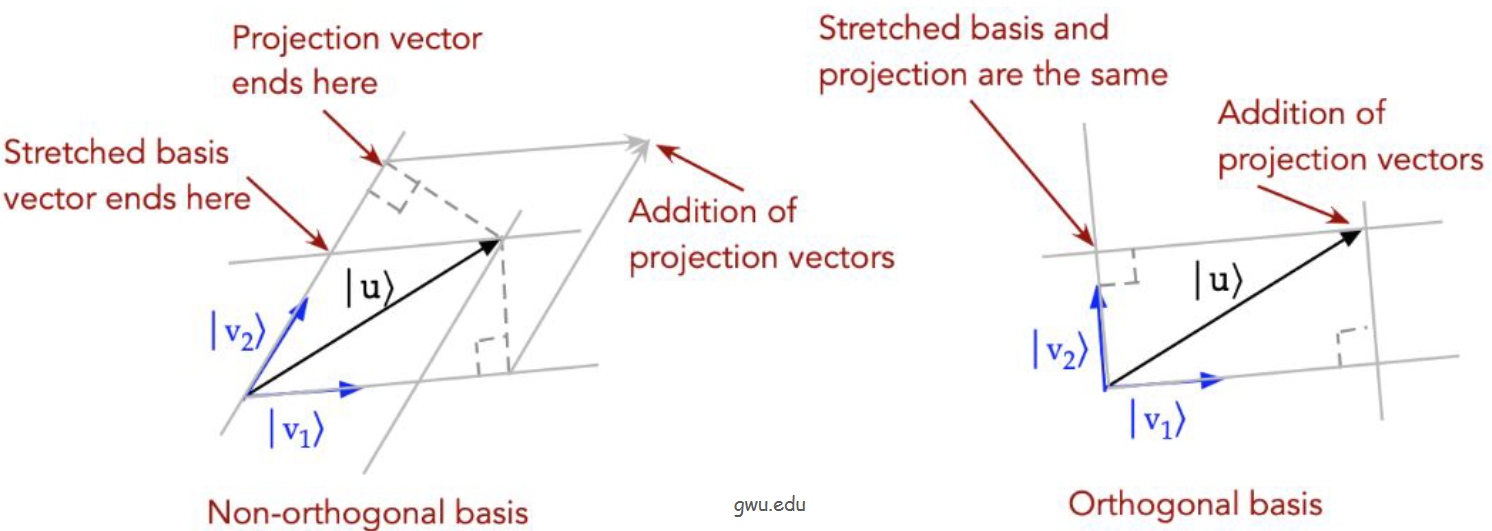
\includegraphics[width=\textwidth]{M9_1.png}
\end{center}
We can also say that a vector $v$ is \textbf{normal} if $\Vert v \Vert_2 = 1$ (graphically it means it lies on the unit (hyper)sphere).\\\\
A basis $B$ is considered an \textbf{orthonormal basis} if 
\begin{enumerate}
	\item $\forall b_i, b_j \in B \::\: b_i b_j = 0$ (meaning all bases are orthogonal)
	\item $\forall b \in B \::\: \Vert b \Vert_2 = 1$ (all vectors are normal).
\end{enumerate}
The nice thing about an orthonormal basis is that when you convert to coordinate representations, you preserve length and angles between vectors.  The most common orthonormal basis for $\mathbb{R}^n$ is the standard basis:
\[\left\{\langle x_1, x_2, \cdots, x_n \rangle \in \mathbb{R}^n \left| \sum_{i = 1}^n x_i = 1, x_i \in \{0, 1\} \forall i \right.\right\}\]
This is, for $\mathbb{R}^3$, the standard basis is $\{\langle 1, 0, 0, \rangle, \langle 0, 1, 0 \rangle, \langle 0, 0, 1 \rangle\}$

\subsubsection*{Multiple Orthonormal Bases}
Notice though that the $\mathbb{R}^2$ standard basis is $\{\langle 1, 0, \rangle, \langle 0, 1 \rangle\}$, we can use a secondary basis:
\[B' = \left\{\left\langle \frac{1}{\sqrt{2}}, \frac{1}{\sqrt{2}}\right\rangle, \left\langle \frac{1}{\sqrt{2}}, -\frac{1}{\sqrt{2}}\right\rangle\right\}\]
is also an orthonormal basis for $\mathbb{R}^2$.\\\\
This means that for any two vectors the coordinate representation of the vectors in both basis will maintain the norms and dot-products.
\begin{itemize}
	\item Intuitively, in this case, we are applying a rotation of the standard basis about the origin to obtain any other orthonormal basis.  This is because orthonormal vectors must have length 1 and be perpendicular to each other.
	\item We are basically rotating our coordinate plane since the basis vectors define it.
	\item As a result, the most that would happen would be all the vectors on the plane are rotated about the origin.  Rotations are linear transformations, which preserve lengths and angles.
\end{itemize}

\subsection*{Matrices as Transformation}
Note that if we construct a matrix $T$ for which the columns are our basis vectors, we can use matrix multiplication to find the coordinate representation: $vT = a$.  So in the example above:
\[T = \begin{bmatrix} \frac{1}{\sqrt{2}} & \frac{1}{\sqrt{2}} \\ \frac{1}{\sqrt{2}} & -\frac{1}{\sqrt{2}} \end{bmatrix}\]
and it follows that 
\[\begin{bmatrix} 6 \\ 2 \end{bmatrix} \begin{bmatrix} \frac{1}{\sqrt{2}} & \frac{1}{\sqrt{2}} \\ \frac{1}{\sqrt{2}} & -\frac{1}{\sqrt{2}} \end{bmatrix} = \begin{bmatrix} 4\sqrt{2} \\ 2\sqrt{2} \end{bmatrix}\]
(We are converting the $\langle 6, 2 \rangle$ in the original coordinate system to the same vector but in terms of the new basis vectors.)\\\\
This will be more useful when talking about eigenelements and decomposition later.

\subsection*{Rank}
Looking back to matrices quickly, remember we can think of a matrix $A \in \mathbb{R}^{n \times m}$ as a set of vectors (either $n$ length $m$ vectors of rows, or $m$ length $n$ vectors of columns).
The \textbf{rank} is the number of linearly independent vectors.  While you may see both row rank and column rank independently, it turns out these are actually always the same.\\\\
For a matrix $A \in \mathbb{R}^{m \times n}$
\begin{itemize}
	\item The rank of a matrix $A$ is denoted as $\text{rk}(A)$, and is defined as the dimension of its column space.  A critical property is that the dimension of the column space is always equal to the dimension of the row space.
	\item Therefore, the rank is also the dimension of the row space.
	\item dim(Column Space) $=$ dim(Row Space) = rk($A$)
	\item This formally explains why "row rank equals column rank" - the number of linearly independent columns is equal to the number of linearly independent rows.
\end{itemize}
We say a matrix is \textbf{full rank} if rank($A$) = min($m, n$).  Notice it is always the case that rank($A$) $\leq$ min($m, n$).  
\begin{itemize}
	\item Because of the property above rk($A$) = rk($AT$), then for some second matrix $B \in \mathbb{R}^{m \times p} \::\:$ rank($AB$) $\leq$ min(rank($A$), rank($B$)).
	\item And for a third matrix $B \in \mathbb{R}^{n \times m} \::\:$ rank($A + B$) $\leq$ rank($A$) + rank($B$).  Note that in the reduced form we talked about previously, the number of non-zero rows is the rank (and the rows are going to be linearly independent).  This also means that any nonsingular (invertible) matrix is full rank (i.e., rank is equal to $n$).
	\item The most common method for calculating rank of a matrix is Gaussian Elimination.  Use row operations to transform the matrix into its row-echelon form.  The rank of the matrix is equal to the number of non-zero rows in its row-echelon form.
\end{itemize}




\end{document}